\documentclass[11pt]{article}

% ---------------------------------------------------------------------------
%  The KT-D1V5 finite-volume discrete Boltzmann solver: method, verification,
%  and comparison with conventional shock-capturing methods.
%  All figures are generated in MATLAB (scripts/make_guide_figures.m) and are
%  stored as .fig/.png/.pdf in the research folder's "figures" directory.
%  Build:  tectonic d1v5_kt_solver_guide.tex
% ---------------------------------------------------------------------------

\usepackage[letterpaper,margin=1in]{geometry}
\usepackage[T1]{fontenc}
\usepackage{lmodern}
\usepackage{microtype}
\usepackage{amsmath,amssymb}
\usepackage{graphicx}
\usepackage{booktabs,tabularx,array}
\usepackage[table]{xcolor}
\usepackage{caption}
\usepackage{enumitem}
\usepackage[numbers,sort&compress]{natbib}
\usepackage[colorlinks=true,linkcolor=blue!45!black,citecolor=blue!45!black,urlcolor=blue!45!black]{hyperref}
\usepackage{cleveref}
\crefname{figure}{Figure}{Figures}\Crefname{figure}{Figure}{Figures}
\crefname{table}{Table}{Tables}\Crefname{table}{Table}{Tables}
\crefname{section}{Section}{Sections}\Crefname{section}{Section}{Sections}
\crefname{equation}{Eq.}{Eqs.}\Crefname{equation}{Eq.}{Eqs.}
\usepackage{tcolorbox}
\tcbuselibrary{breakable}
\usepackage{float}
\usepackage{fancyhdr}
\usepackage{titlesec}

\graphicspath{{../figures/}}
\captionsetup{font=small,labelfont=bf,labelsep=period}
\setlist{itemsep=2pt,topsep=3pt}
\setlength{\parskip}{3pt}
\titleformat{\section}{\large\bfseries}{\thesection}{0.8em}{}
\titleformat{\subsection}{\normalsize\bfseries}{\thesubsection}{0.8em}{}

\pagestyle{fancy}
\fancyhf{}
\lhead{\small KT-D1V5 Finite-Volume Discrete Boltzmann Solver}
\rhead{\small N.\ Kidwell}
\cfoot{\small\thepage}
\renewcommand{\headrulewidth}{0.4pt}

\newcommand{\feq}{f^{\mathrm{eq}}}
\makeatletter
\newcommand{\tabinput}[1]{\@@input #1 }
\makeatother

% key-point box and figure-discussion box
\newtcolorbox{keypoint}[1][]{colback=blue!3,colframe=blue!40!black,boxrule=0.5pt,arc=1.5pt,
  left=6pt,right=6pt,top=4pt,bottom=4pt,fonttitle=\bfseries\small,title=#1}
\newtcolorbox{figexplain}[1]{breakable,colback=gray!4,colframe=gray!55,boxrule=0.4pt,arc=1pt,
  left=6pt,right=6pt,top=3pt,bottom=3pt,fonttitle=\bfseries\small,coltitle=black,colbacktitle=gray!15,title={Discussion of #1}}
\newlist{fx}{description}{1}
\setlist[fx]{font=\normalfont\itshape,leftmargin=0pt,itemsep=2pt,topsep=1pt}

\begin{document}

% ------------------------------------------------------------------ title
\begin{center}
{\Large\bfseries The KT-D1V5 Finite-Volume Discrete Boltzmann Solver}\\[6pt]
{\large Method, Verification on the Sod Shock Tube, and Comparison with\\ Conventional Shock-Capturing Schemes}\\[14pt]
{\normalsize Nathan Kidwell}\\[2pt]
{\small Embry-Riddle Aeronautical University \quad$\cdot$\quad September 2026}
\end{center}

\vspace{4pt}
\begin{tcolorbox}[colback=white,colframe=black!60,boxrule=0.5pt,arc=0pt,left=8pt,right=8pt]
\small\textbf{Abstract.}\;
This report describes a one-dimensional finite-volume discrete Boltzmann method (FVDBM)
for compressible flow and evaluates it on the Sod shock tube.  The gas is represented by
five discrete particle populations (the Kataoka--Tsutahara D1V5 model) that are transported
through a finite-volume grid and relaxed toward a local equilibrium by a BGK collision term.
Spatial accuracy is provided by MUSCL reconstruction with a generalized-minmod limiter
($\theta = 1.2$), and time integration by a three-stage strong-stability-preserving
Runge--Kutta scheme.  On five grids from 3{,}125 to 50{,}000 cells the solution converges
without oscillation, conserves mass and energy to $10^{-12}$, and shows observed orders of
0.81--0.89 in the $L_1$ norm and 0.40--0.63 in the $L_2$ norm.  These rates are below the
smooth-flow values of 1 (first order) and 2 (second order), as the theory for solutions
containing a shock and a contact discontinuity predicts for every shock-capturing method.
The solver is compared, on identical grids, with first-order and other limited versions of
itself and with a conventional finite-volume Euler solver.  At equal resolution the
DBM and a conventional second-order Euler solver reach similar accuracy and convergence
rates, clearly better than first-order methods, but the DBM requires 100 to 800 times more
computing time because its explicit collision term limits the time step to one quarter of
the relaxation time.
\end{tcolorbox}

\vspace{2pt}
{\small\tableofcontents}
\clearpage

% ===========================================================================
\section{Introduction}
% ===========================================================================

Discrete Boltzmann methods (DBMs) model a gas with a small number of particle
populations rather than solving the fluid equations directly.  The macroscopic
density, velocity, temperature and pressure are obtained as sums (moments) of the
populations, and the familiar Euler equations are recovered when collisions are
frequent~\citep{KataokaTsutahara2004Euler,XuZhangZhang2018}.  The approach is attractive
because the same populations also carry information about departures from
thermodynamic equilibrium, which conventional Euler or Navier--Stokes solvers do not
represent.

The solver examined here solves the one-dimensional Sod shock tube~\citep{Sod1978}, a
standard benchmark whose exact solution contains the three basic wave types of gas
dynamics.  The objectives of this report are to
\begin{enumerate}
  \item describe the physical model and the numerical method in a concise, self-contained way;
  \item quantify the accuracy of the solver and state clearly what order of accuracy the
        measurements indicate;
  \item compare its accuracy and computational cost with alternative methods run on the
        same problem and grids; and
  \item explain each figure and what it implies for the method.
\end{enumerate}
All figures were produced in MATLAB and are stored, in \texttt{.fig}, \texttt{.png} and
\texttt{.pdf} form, in the \texttt{figures} folder of the research directory.

\paragraph{Configuration.}  Unless stated otherwise, all results use the settings in
\cref{tab:config}.

\begin{table}[H]
\centering
\caption{Solver configuration.}
\label{tab:config}
\small
\begin{tabular}{@{}lll@{}}
\toprule
Parameter & Symbol & Value \\
\midrule
Ratio of specific heats & $\gamma$ & 1.4 \\
Relaxation time & $\tau$ & $5\times10^{-6}$ \\
Discrete speeds & $c_i$ & $0,\ \pm1,\ \pm3$ \\
Internal-energy parameter & $\eta_0$ & 1.75 \\
Domain length, diaphragm position & $L_x$, $x_0$ & 20, 10 \\
Final time & $t_{\mathrm{end}}$ & 0.15 \\
Slope limiter & generalized minmod & $\theta = 1.2$ \\
Time integrator & SSP-RK3 & $\Delta t = \min(\mathrm{CFL}\,\Delta x/3,\ \tau/4)$, CFL $=0.025$ \\
Grids & $N_x$ & 3{,}125;\ 6{,}250;\ 12{,}500;\ 25{,}000;\ 50{,}000 \\
Boundary condition & --- & zero gradient (transmissive) \\
\bottomrule
\end{tabular}
\end{table}

% ===========================================================================
\section{Test problem: the Sod shock tube}
\label{sec:sod}
% ===========================================================================

A tube of length 20 contains two gases separated by a diaphragm at $x_0 = 10$.  The
initial states are
\[
(\rho,\,u,\,p) = (1,\,0,\,1) \ \ \text{for } x<x_0,
\qquad
(\rho,\,u,\,p) = (0.125,\,0,\,0.1) \ \ \text{for } x>x_0,
\]
where $\rho$ is density, $u$ velocity and $p$ pressure (nondimensional, with $p=\rho T$).
When the diaphragm is removed three waves form: a \emph{rarefaction} travelling left, a
\emph{contact discontinuity} travelling right with the gas, and a \emph{shock} travelling
right ahead of it.  The exact solution is obtained from the Riemann problem for the Euler
equations~\citep{Toro2009}; its key values are listed in \cref{tab:sod}.

\begin{table}[H]
\centering
\caption{Exact solution at $t = 0.15$.}
\label{tab:sod}
\small
\begin{tabular}{@{}lll@{}}
\toprule
Quantity & Value & Remark \\
\midrule
Pressure and velocity between the waves & $p^* = 0.3031$, $u^* = 0.9275$ & continuous across the contact \\
Density on either side of the contact & $0.4263$ / $0.2656$ & jump of 0.161 \\
Temperature on either side of the contact & $0.711$ / $1.141$ & jump of 0.430 \\
Shock speed (Mach number) & 1.752 (1.66) & position $x_0 + 0.263$ \\
Contact position & $x_0 + 0.139$ & moves at $u^*$ \\
Rarefaction extent & $x_0 - 0.177$ to $x_0 - 0.011$ & smooth \\
\bottomrule
\end{tabular}
\end{table}

\begin{figure}[H]
\centering
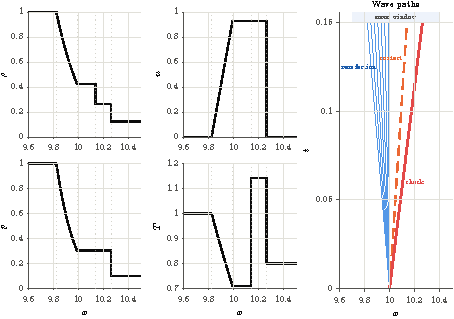
\includegraphics[width=\textwidth]{G02_exact_sod.pdf}
\caption{Exact solution of the Sod problem at $t=0.15$ (left) and the space--time paths of
the three waves (right).}
\label{fig:exact}
\end{figure}

\begin{figexplain}{\Cref{fig:exact}}
\begin{fx}
\item[What is shown.] The four panels on the left give density, velocity, pressure and
  temperature along the tube at the final time; dotted vertical lines mark the head and
  tail of the rarefaction, the contact and the shock.  The right panel traces each wave
  in the $x$--$t$ plane, starting from the diaphragm at $x = 10$, $t = 0$.
\item[How to read it.] In the wave diagram, the fan of thin blue lines is the rarefaction,
  the dashed orange line is the contact and the thick red line is the shock; steeper lines
  are slower waves.  The shaded strip at the top marks the region $9.7 \le x \le 10.4$ used
  for the wave-region error measurements.
\item[What it means.] The problem tests three distinct behaviours at once: a smooth
  expansion, a density/temperature jump with no pressure change (contact), and a jump in
  every variable (shock).  Numerical methods typically handle these very differently, and
  the contact is usually the most difficult to keep sharp.
\end{fx}
\end{figexplain}

% ===========================================================================
\section{Physical model}
\label{sec:model}
% ===========================================================================

\subsection{Kinetic description}
Instead of the fluid variables, the solver evolves a set of particle populations $f_i(x,t)$,
each moving at a fixed speed $c_i$.  Each population obeys the discrete BGK equation
\begin{equation}
  \frac{\partial f_i}{\partial t} + c_i\,\frac{\partial f_i}{\partial x}
  = \frac{\feq_i - f_i}{\tau}, \qquad i = 1,\dots,5 .
  \label{eq:dbe}
\end{equation}
The left-hand side describes free streaming of population $i$ along the tube.  The
right-hand side is the Bhatnagar--Gross--Krook (BGK) collision model~\citep{BGK1954}: collisions
relax each population toward a local equilibrium $\feq_i$ at a rate set by the relaxation
time $\tau$, which can be interpreted as the mean time between collisions.  For small
$\tau$ the populations remain close to equilibrium and their moments satisfy the Euler
equations~\citep{ChapmanCowling1970}.

\subsection{The D1V5 velocity set}
The model uses one spatial dimension and five velocities (D1V5), following Kataoka and
Tsutahara~\citep{KataokaTsutahara2004Euler}:
\[
c_i \in \{-3,\ -1,\ 0,\ +1,\ +3\}.
\]
The stationary population is assigned an internal-energy parameter $\eta_0 = 1.75$.  This
represents the rotational and transverse energy of real molecules and allows the model to
reproduce a gas with $\gamma = 1.4$.

\begin{figure}[H]
\centering
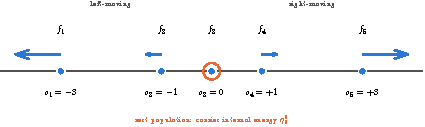
\includegraphics[width=0.85\textwidth]{G01_velocity_set.pdf}
\caption{The five discrete velocities of the D1V5 model.}
\label{fig:velset}
\end{figure}

\begin{figexplain}{\Cref{fig:velset}}
\begin{fx}
\item[What is shown.] Each dot is one population $f_i$ placed at its velocity $c_i$; arrows
  indicate direction and relative speed.  The circled centre population is stationary.
\item[What it means.] Two populations move left, two move right and one is at rest.  The
  fastest speed, 3, sets the transport time-step limit (\cref{sec:time}).  Because the
  stationary population carries the internal energy, the model can represent a diatomic
  gas with only five populations.
\end{fx}
\end{figexplain}

\subsection{Equilibrium distribution}
The equilibrium populations $\feq_i(\rho,u,T)$ are determined by requiring that they
reproduce exactly five quantities: density, momentum, total energy, and the fluxes of
momentum and energy that appear in the Euler equations.  Five conditions on five unknowns
give a unique solution, which is the explicit formula used by the solver.  This equilibrium
was verified numerically to reproduce all five quantities to machine precision
($\approx10^{-15}$) over 2000 random states.

\begin{figure}[H]
\centering
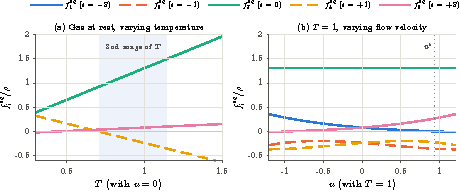
\includegraphics[width=\textwidth]{G03_equilibrium.pdf}
\caption{Equilibrium populations per unit density as functions of temperature (a) and flow
velocity (b).}
\label{fig:feq}
\end{figure}

\begin{figexplain}{\Cref{fig:feq}}
\begin{fx}
\item[What is shown.] Panel (a) shows the five equilibrium values for a gas at rest as the
  temperature varies; the shaded band marks the temperatures that occur in the Sod
  solution.  Panel (b) holds $T = 1$ and varies the flow velocity.
\item[How to read it.] In (a) the left- and right-moving pairs coincide because the gas is
  at rest.  In (b) a positive velocity increases the right-moving populations and decreases
  the left-moving ones, which is how momentum is represented.
\item[What it means.] The slow populations ($c=\pm1$) are \emph{negative} over most of the
  Sod temperature range.  This is permissible because the populations are moment carriers
  rather than physical particle counts, but it means positivity cannot be enforced on the
  individual $f_i$; the solver instead checks that the recovered density and temperature
  remain positive.  Panel (b) also shows that near the post-shock velocity $u^*$ the fast
  population moving against the flow approaches zero.
\end{fx}
\end{figexplain}

\subsection{Recovery of the macroscopic variables}
The fluid variables in each cell are weighted sums of the five populations:
\begin{equation}
\rho = \sum_i f_i, \qquad
\rho u = \sum_i c_i f_i, \qquad
\rho\,(bT + u^2) = \sum_i \bigl(c_i^2 + \eta_i^2\bigr) f_i, \qquad
p = \rho T,
\label{eq:moments}
\end{equation}
with $b = 2/(\gamma-1) = 5$.  Temperature is obtained by subtracting the kinetic-energy
contribution $u^2$ from the total energy.  Because it is the difference of two larger
quantities, temperature is the variable most sensitive to small errors in individual
populations, particularly the fast ones.  This is why numerical overshoots appear first in
the temperature profile (\cref{sec:limiters}).

Collisions conserve mass, momentum and energy exactly, since the equilibrium is
constructed from the same totals as the current populations.

\subsection{Effect of the relaxation time}
The exact Sod solution assumes an inviscid gas ($\tau = 0$), whereas the model uses a small
but finite $\tau$.  A first-order (Chapman--Enskog) analysis of the D1V5 model shows that
finite $\tau$ has two practical consequences:
\begin{itemize}
  \item The physical shock thickness is approximately $7\tau \approx 4\times10^{-5}$, well
        below the finest cell size ($4\times10^{-4}$).  The computed shock width is
        therefore set by the grid, not by $\tau$.
  \item The contact diffuses with time, like heat conduction, and reaches a physical width
        of about $1.2$--$1.5\times10^{-3}$ at $t = 0.15$ (about three cells on the finest
        grid).  Grid refinement beyond this scale cannot sharpen the contact further.
\end{itemize}
The same analysis shows that the diffusion rate at a contact depends on the local flow
speed and would become negative (unstable) if the flow speed exceeded the slow particle
speed of 1.  The D1V5 velocity set is therefore suited to flows with velocities below this
value; the Sod problem ($u^* = 0.93$) lies just inside this limit.

% ===========================================================================
\section{Numerical method}
\label{sec:method}
% ===========================================================================

\subsection{Finite-volume discretization}
The tube is divided into $N_x$ cells of width $\Delta x = L_x/N_x$.  Each cell stores the
cell-averaged value of every population.  Integrating \cref{eq:dbe} over a cell gives
\begin{equation}
\frac{\mathrm{d}f_{i,j}}{\mathrm{d}t}
= -\frac{F_{i,j+1/2} - F_{i,j-1/2}}{\Delta x} + \frac{\feq_{i,j} - f_{i,j}}{\tau},
\label{eq:fv}
\end{equation}
where $F_{i,j\pm1/2}$ is the flux of population $i$ through the right and left faces of cell $j$.
Because the flux leaving one cell enters its neighbour, the scheme is conservative by
construction; the results confirm conservation of mass and energy to $\approx10^{-12}$.

\subsection{Upwind fluxes and MUSCL reconstruction}
Each population moves in a single direction, so the flux at a face is taken from the
upstream side (upwinding): populations with $c_i > 0$ use the value reconstructed from the
cell on the left of the face, those with $c_i < 0$ use the value from the right, and the
stationary population has no flux.  For linear advection this upwind choice is the exact
solution of the local Riemann problem.

Using the cell average itself at the face gives a first-order scheme that is robust but
strongly diffusive.  MUSCL reconstruction~\citep{vanLeer1979} instead represents the data in
each cell by a straight line of slope $\sigma_j$ and evaluates that line at the faces:
\begin{equation}
f^{-}_{j+1/2} = f_j + \tfrac12\sigma_j, \qquad f^{+}_{j+1/2} = f_{j+1} - \tfrac12\sigma_{j+1}.
\label{eq:muscl}
\end{equation}
With an accurate slope, the leading diffusive error of the first-order scheme cancels and
the method becomes second-order accurate in smooth regions.

\begin{figure}[H]
\centering
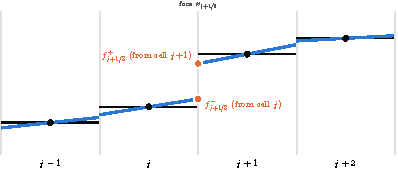
\includegraphics[width=0.85\textwidth]{G04_muscl_schematic.pdf}
\caption{MUSCL reconstruction for one population on four cells.}
\label{fig:muscl}
\end{figure}

\begin{figexplain}{\Cref{fig:muscl}}
\begin{fx}
\item[What is shown.] Black horizontal segments are the stored cell averages; blue lines are
  the limited linear reconstructions within each cell; the two orange points are the two
  candidate values at the face between cells $j$ and $j+1$.
\item[How to read it.] A right-moving population takes the lower orange value
  $f^-_{j+1/2}$ (from cell $j$); a left-moving population takes the upper value
  $f^+_{j+1/2}$ (from cell $j+1$).  The gap between the two values is largest where the data
  change rapidly.
\item[What it means.] Compared with a first-order method, which would use the flat black
  values, the sloped reconstruction places a more accurate value at each face and greatly
  reduces numerical smearing.  The slope must be limited near jumps to avoid creating new
  maxima or minima, which is the role of the limiter described next.
\end{fx}
\end{figexplain}

\subsection{Generalized-minmod slope limiter}
\label{sec:limiter}
Let $d_L = f_j - f_{j-1}$ and $d_R = f_{j+1} - f_j$.  The slope is
\begin{equation}
\sigma_j = \operatorname{minmod}\!\Bigl(\theta d_L,\ \tfrac12(d_L + d_R),\ \theta d_R\Bigr),
\qquad 1 \le \theta \le 2,
\label{eq:gminmod}
\end{equation}
where $\operatorname{minmod}$ returns the argument of smallest magnitude if all arguments
share the same sign, and zero otherwise~\citep{KurganovTadmor2000}.  The parameter $\theta$
controls how aggressive the reconstruction is: $\theta = 1$ reproduces the minmod limiter
(most dissipative) and $\theta = 2$ the monotonized-central (MC) limiter~\citep{vanLeer1977}
(sharpest).  The solver uses $\theta = 1.2$.  For $1 \le \theta \le 2$ the scheme is
total-variation diminishing (TVD) for each population's transport, meaning that it cannot
create new oscillations~\citep{Harten1983,Sweby1984}.

\begin{figure}[H]
\centering
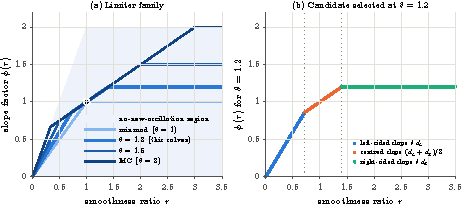
\includegraphics[width=\textwidth]{G05_limiters.pdf}
\caption{Generalized-minmod limiter functions (a) and the candidate slope selected at
$\theta=1.2$ (b).}
\label{fig:limiters}
\end{figure}

\begin{figexplain}{\Cref{fig:limiters}}
\begin{fx}
\item[What is shown.] The horizontal axis is the smoothness ratio $r = d_L/d_R$, which equals
  1 for perfectly linear data and is negative at a local maximum or minimum.  The vertical
  axis is the fraction $\phi(r) = \sigma/d_R$ of the right-hand difference used as the slope.
  The shaded area is the region in which a limiter is guaranteed not to create new
  oscillations.
\item[How to read it.] Higher curves allow steeper slopes (sharper results).  All curves pass
  through $\phi(1) = 1$, so linear data are reproduced exactly.  Panel (b) colours the
  $\theta = 1.2$ curve by which of the three candidate slopes in \cref{eq:gminmod} is chosen.
\item[What it means.] $\theta = 1.2$ lies only slightly above minmod: it permits slopes up to
  20\% steeper than a one-sided difference and uses the centred slope for moderately smooth
  data ($0.71 < r < 1.4$).  This yields a modest gain in sharpness over minmod while
  remaining far from the aggressive MC limiter, which is the source of the temperature
  overshoot discussed in \cref{sec:limiters}.
\end{fx}
\end{figexplain}

\subsection{Time integration and time-step selection}
\label{sec:time}
The semi-discrete system \cref{eq:fv} is advanced with the three-stage, third-order
strong-stability-preserving Runge--Kutta (SSP-RK3) scheme of Shu and Osher~\citep{ShuOsher1988,Gottlieb2001}:
\begin{align*}
f^{(1)} &= f^n + \Delta t\,\mathcal{L}(f^n),\\
f^{(2)} &= \tfrac34 f^n + \tfrac14\bigl[f^{(1)} + \Delta t\,\mathcal{L}(f^{(1)})\bigr],\\
f^{n+1} &= \tfrac13 f^n + \tfrac23\bigl[f^{(2)} + \Delta t\,\mathcal{L}(f^{(2)})\bigr],
\end{align*}
where $\mathcal{L}$ denotes the right-hand side of \cref{eq:fv}.  Each stage is a weighted
average of forward-Euler steps, so the non-oscillatory property of the spatial scheme is
preserved.

The time step is the smaller of a transport limit and a collision limit:
\begin{equation}
\Delta t = \min\Bigl(\mathrm{CFL}\,\frac{\Delta x}{\max|c_i|},\ \ \frac{\tau}{4}\Bigr).
\label{eq:dt}
\end{equation}
With $\tau = 5\times10^{-6}$ the collision limit gives $\Delta t = 1.25\times10^{-6}$, which
is smaller than the transport limit on every grid.  All runs therefore use the same
$\Delta t$ and 120{,}000 time steps, and the effective transport Courant number is only
$6\times10^{-4}$ to $9\times10^{-3}$.  This restriction is the dominant factor in the
computational cost of the method (\cref{sec:comparison}).

\subsection{Robustness safeguards}
After each Runge--Kutta stage the solver checks that density and temperature are positive
and finite.  A failed stage is repeated with half the time step and, if necessary, with a
more dissipative limiter.  No retries or limiter fallbacks occurred in any run reported
here, so all results are those of the unmodified scheme.

% ===========================================================================
\section{Accuracy assessment}
\label{sec:metrics}
% ===========================================================================

At every cell the computed value $q_j$ is compared with the exact value $q_j^{\mathrm{ex}}$:
\begin{equation}
L_1 = \frac{1}{N_x}\sum_j |q_j - q_j^{\mathrm{ex}}|, \qquad
L_2 = \Bigl[\frac{1}{N_x}\sum_j (q_j - q_j^{\mathrm{ex}})^2\Bigr]^{1/2}.
\end{equation}
$L_1$ is the mean absolute error; $L_2$ is the root-mean-square error, which weights large
local errors more heavily.  If the error behaves as $E \approx C\,\Delta x^{p}$, the
\emph{observed order} $p$ between two grids is
\begin{equation}
p = \frac{\ln(E_{\text{coarse}}/E_{\text{fine}})}{\ln(\Delta x_{\text{coarse}}/\Delta x_{\text{fine}})},
\end{equation}
and a least-squares fit of $\ln E$ against $\ln\Delta x$ gives the order over all grids.
Halving the cell size halves the error for $p = 1$ (first order) and quarters it for $p = 2$
(second order).

\begin{keypoint}[What order should be expected on this problem?]
The formal order of a method (1 for first-order upwind, 2 for MUSCL) applies only to smooth
solutions.  A discontinuity is always smeared over a few cells, so the error there does not
shrink as quickly.  For methods of this type the expected orders on the Sod problem
are~\citep{Harten1977,LeVeque2002,Greenough2004}:
\begin{center}
\small
\begin{tabular}{@{}lcccc@{}}
\toprule
 & \multicolumn{2}{c}{Smooth solution} & \multicolumn{2}{c}{With shock and contact} \\
\cmidrule(lr){2-3}\cmidrule(l){4-5}
Method & $L_1$ & $L_2$ & $L_1$ & $L_2$ \\
\midrule
First order & 1 & 1 & 0.5 (contact) to 1 (shock) & 0.25 to 0.5 \\
Second order (MUSCL) & 2 & 2 & 0.67 (contact) to 1 (shock) & 0.33 to 0.5 \\
\bottomrule
\end{tabular}
\end{center}
Asymptotically, an $L_1$ order near 1 and an $L_2$ order near 0.5 is the best that any
shock-capturing method, of any formal order, can achieve on this problem; on finite grids
the measured values can differ somewhat from these limits.
\end{keypoint}

% ===========================================================================
\section{Results}
\label{sec:results}
% ===========================================================================

\subsection{Solution on the finest grid}

\begin{figure}[H]
\centering
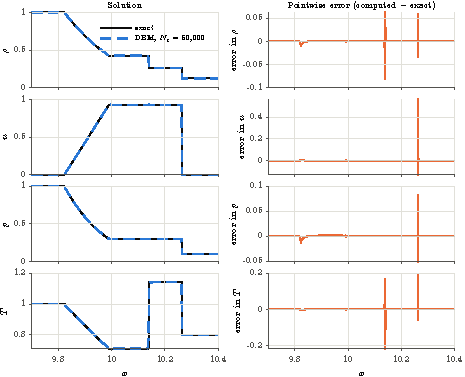
\includegraphics[width=\textwidth]{G06_finest_solution.pdf}
\caption{Computed solution on 50{,}000 cells compared with the exact solution (left), and
the pointwise error (right).}
\label{fig:finest}
\end{figure}

\begin{figexplain}{\Cref{fig:finest}}
\begin{fx}
\item[What is shown.] The left column overlays the computed density, velocity, pressure and
  temperature (dashed blue) on the exact solution (black) in the region containing the
  waves.  The right column plots the difference between them at each cell.
\item[How to read it.] Where the curves on the left coincide, the error on the right is
  zero.  Spikes in the error column mark locations where the computed profile is slightly
  displaced or rounded relative to the exact jump.
\item[What it means.] The computed solution matches the exact one closely in all four
  variables and contains no spurious oscillations.  The error is confined to a few cells at
  the contact (density and temperature) and at the shock (all variables), with small
  deviations at the corners of the rarefaction.  The peak pointwise error does not vanish
  under refinement because a jump spread over a few cells always leaves an $O(1)$ error in
  the cells that straddle it; the average errors ($L_1$, $L_2$) nonetheless decrease, as
  shown below.
\end{fx}
\end{figexplain}

\subsection{Effect of grid refinement}

\begin{figure}[H]
\centering
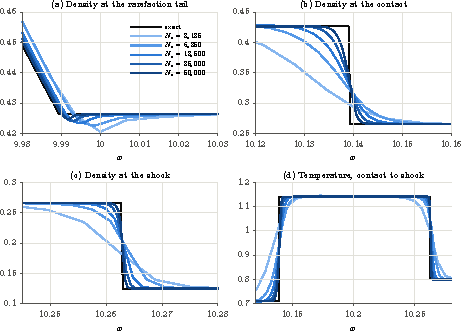
\includegraphics[width=\textwidth]{G07_grid_zoom.pdf}
\caption{Close-up views of each wave on the five grids.  Darker curves correspond to finer
grids.}
\label{fig:zoom}
\end{figure}

\begin{figexplain}{\Cref{fig:zoom}}
\begin{fx}
\item[What is shown.] Magnified views of (a) the tail of the rarefaction, (b) the contact,
  (c) the shock and (d) the temperature between the contact and the shock, for all five
  grids.
\item[How to read it.] The black line is the exact solution; the lightest blue curve is the
  coarsest grid (3{,}125 cells) and the darkest is the finest (50{,}000 cells).  A sharper
  step and a curve closer to black indicate higher accuracy.
\item[What it means.] Every refinement sharpens every wave.  The shock (c) occupies roughly
  three cells on every grid, so its physical width halves with each refinement.  The contact
  (b) narrows more slowly and spreads over more cells as the grid is refined, which is
  characteristic of contact discontinuities.  A small temperature overshoot visible on the
  coarsest grids in (d) disappears by 12{,}500 cells.  A slight undershoot below the tail of
  the rarefaction (a) also diminishes with refinement.
\end{fx}
\end{figexplain}

\subsection{Convergence and order of accuracy}
\label{sec:convergence}

\begin{table}[H]
\centering
\caption{Global errors of the DBM solver ($\theta = 1.2$) and observed orders from a
least-squares fit over all five grids.}
\label{tab:conv}
\small
\begin{tabular}{@{}rcccccccc@{}}
\toprule
 & \multicolumn{4}{c}{$L_1$ error} & \multicolumn{4}{c}{$L_2$ error} \\
\cmidrule(lr){2-5}\cmidrule(l){6-9}
$N_x$ & $\rho$ & $u$ & $p$ & $T$ & $\rho$ & $u$ & $p$ & $T$ \\
\midrule
3,125  & 2.46e-4 & 4.14e-4 & 2.14e-4 & 3.58e-4 & 3.16e-3 & 7.79e-3 & 3.08e-3 & 5.92e-3 \\
6,250  & 1.30e-4 & 2.69e-4 & 1.09e-4 & 2.08e-4 & 1.81e-3 & 8.06e-3 & 1.64e-3 & 4.65e-3 \\
12,500 & 7.23e-5 & 1.43e-4 & 5.75e-5 & 1.17e-4 & 1.39e-3 & 6.13e-3 & 1.14e-3 & 3.54e-3 \\
25,000 & 4.07e-5 & 6.29e-5 & 3.11e-5 & 6.36e-5 & 1.00e-3 & 2.71e-3 & 7.20e-4 & 2.44e-3 \\
50,000 & 2.51e-5 & 3.97e-5 & 1.88e-5 & 3.98e-5 & 7.77e-4 & 2.75e-3 & 5.15e-4 & 2.02e-3 \\
\midrule
Observed order & 0.83 & 0.89 & 0.88 & 0.81 & 0.49 & 0.46 & 0.63 & 0.40 \\
\bottomrule
\end{tabular}
\end{table}

\begin{figure}[H]
\centering
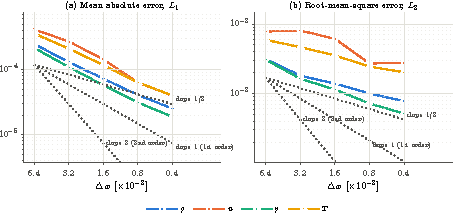
\includegraphics[width=\textwidth]{G08_convergence.pdf}
\caption{Convergence of the $L_1$ (a) and $L_2$ (b) errors of the DBM solver.  Dotted lines
show reference slopes of 2 (second order), 1 (first order) and $1/2$.}
\label{fig:conv}
\end{figure}

\begin{figexplain}{\Cref{fig:conv}}
\begin{fx}
\item[What is shown.] The error in each variable plotted against cell size on logarithmic
  axes, with the finest grid on the right.  On such a plot a method of order $p$ appears as
  a straight line of slope $p$.
\item[How to read it.] Compare the slope of each data line with the dotted reference lines.
  A line parallel to ``slope 2'' would indicate second-order convergence; parallel to
  ``slope 1'', first order.
\item[What it means.] All four $L_1$ curves fall with a slope just below 1, and the $L_2$
  curves with slopes between about 0.4 and 0.6, between the ``slope 1/2'' and ``slope 1''
  references.  Both sets are close to the best possible rates for a solution containing a
  shock and a contact (\cref{sec:metrics}).  The velocity curve in (b) levels off between
  the two finest grids; \cref{sec:phase} shows that this is a measurement effect.
\end{fx}
\end{figexplain}

\begin{keypoint}[Does the $L_2$ error indicate a first-order or a second-order solution?]
The measured $L_2$ orders are \textbf{0.40 to 0.63}, and the $L_1$ orders are \textbf{0.81
to 0.89}.  Taken at face value, both are \emph{below first order}; neither norm shows
second-order convergence.  This does not mean the method is less accurate than a
first-order scheme.  The reconstruction is formally second order, but on a problem with
discontinuities every shock-capturing scheme is asymptotically limited to an $L_1$ order of
about 1 and an $L_2$ order of about $1/2$, and the contact lowers these further.  The
measured values should therefore be judged against other methods on the same problem
rather than against the smooth-flow values of 1 and 2.  \Cref{sec:comparison} does this
directly: on the same grids a first-order version of the solver converges with $L_1$ order
0.64, while the present solver (0.86) matches a conventional second-order Euler solver
(0.92).  The solver therefore behaves as a \emph{second-order} method would on this
problem: clearly better than first order, but, like every shock-capturing scheme, well below
the formal rate of 2.
\end{keypoint}

% ---------------------------------------------------------------------------
% Comparison with other methods (accuracy and computational cost).
% Table rows in data/tab_methods.tex are written by make_guide_figures.m.
% ---------------------------------------------------------------------------
\subsection{Comparison with other methods: accuracy and computational cost}
\label{sec:comparison}

To place the solver in context, the same Sod problem was solved on the same grids with
five alternative methods:
\begin{itemize}
  \item the \textbf{same DBM} with three other reconstructions: first-order upwind (no
        slope), MUSCL with minmod, and MUSCL with MC; and
  \item a \textbf{conventional finite-volume Euler solver}, which evolves density,
        momentum and energy directly, using the HLLC approximate Riemann
        solver~\citep{ToroSpruceSpeares1994,Toro2009} with either first-order reconstruction
        or the same generalized-minmod MUSCL reconstruction ($\theta = 1.2$) and SSP-RK3
        time stepping at a standard CFL number of 0.5.
\end{itemize}
All computations used the same computer, one processor core and MATLAB R2024b.  The Euler
times are the best of three measured runs.  The DBM times are the measured cost per cell per
time step ($4.05\times10^{-7}$\,s for MUSCL and $2.74\times10^{-7}$\,s for first order,
obtained from isolated runs on the two coarsest grids) multiplied by the number of cells and
time steps; this cost was verified to be the same on both grids to within 0.4\%.

\begin{table}[H]
\centering
\caption{Accuracy and cost of the six methods.  Orders are least-squares fits over the grids
3{,}125--25{,}000 (common to all methods); errors and cost are for 25{,}000 cells.}
\label{tab:methods}
\small
\begin{tabular}{@{}lcccccc@{}}
\toprule
 & \multicolumn{2}{c}{Observed order ($\rho$)} & \multicolumn{2}{c}{Error at 25{,}000 cells} & \multicolumn{2}{c}{Cost at 25{,}000 cells} \\
\cmidrule(lr){2-3}\cmidrule(lr){4-5}\cmidrule(l){6-7}
Method & $L_1$ & $L_2$ & $L_1(\rho)$ & $L_2(\rho)$ & time steps & time [s] \\
\midrule
\tabinput{data/tab_methods.tex}
\bottomrule
\end{tabular}
\end{table}

\begin{figure}[H]
\centering
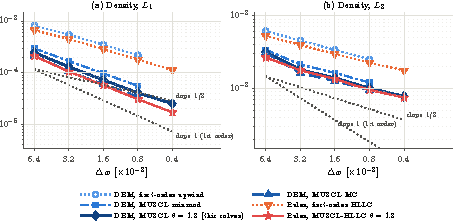
\includegraphics[width=\textwidth]{G09_order_comparison.pdf}
\caption{Density error versus cell size for the six methods: $L_1$ (a) and $L_2$ (b).}
\label{fig:ordercomp}
\end{figure}

\begin{figexplain}{\Cref{fig:ordercomp}}
\begin{fx}
\item[What is shown.] The density error of every method on every grid.  Blue curves are
  DBM variants (the dark solid curve is the solver studied here); red and orange curves are
  the conventional Euler solver.  Hollow markers denote first-order methods.
\item[How to read it.] Lower curves are more accurate at a given grid; steeper curves improve
  faster with refinement.  The dotted lines give reference slopes of 1 and $1/2$.
\item[What it means.] The methods separate into two groups.  The two first-order methods
  (hollow markers) have errors three to seven times larger, with the gap widening under
  refinement, and converge more slowly ($L_1$ order 0.64).  All second-order methods cluster together with $L_1$ orders of
  0.80--0.92, whether they are kinetic (DBM) or conventional (Euler).  At equal resolution
  the density error of the present DBM is about one third larger than that of the
  conventional MUSCL-HLLC solver.  The order of accuracy is therefore determined by the
  reconstruction, not by whether the gas is modelled kinetically or with the Euler equations.
\end{fx}
\end{figexplain}

\begin{figure}[H]
\centering
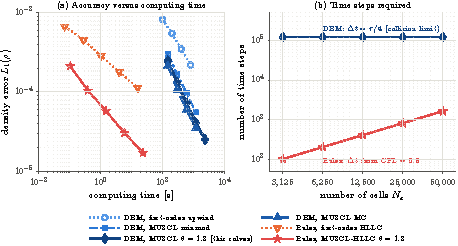
\includegraphics[width=\textwidth]{G10_accuracy_vs_cost.pdf}
\caption{(a) Density error versus computing time for the six methods.  (b) Number of time
steps required by the DBM and the Euler solver on each grid.}
\label{fig:cost}
\end{figure}

\begin{figexplain}{\Cref{fig:cost}}
\begin{fx}
\item[What is shown.] Panel (a) is a work--precision diagram: each point is one grid, placed by
  its computing time (horizontal) and its density error (vertical).  Panel (b) shows how many
  time steps each solver needed on each grid.
\item[How to read it.] In (a), the most efficient method is the one whose curve lies furthest to
  the lower left, meaning the lowest error for a given time.  A horizontal line through the
  plot compares the time each method needs to reach the same error.
\item[What it means.] The conventional Euler solvers are two to three orders of magnitude
  faster than the DBM for the same accuracy.  Panel (b) explains why.  The cost per cell per
  time step is similar for both solvers ($4.1\times10^{-7}$\,s for the DBM versus about
  $2.9\times10^{-7}$\,s for MUSCL-HLLC), but the DBM needs 120{,}001 steps on every grid
  because its time step is fixed by the collision limit $\Delta t = \tau/4$, whereas the Euler
  solver's step is set by the wave speed and needs only 102 steps on the coarsest grid and
  1{,}643 on the finest.  The gap therefore narrows with refinement, from about 780 times at
  6{,}250 cells to about 100 times at 50{,}000 cells.
\end{fx}
\end{figexplain}

\paragraph{Quantitative summary.}
\begin{itemize}
  \item \textbf{Second-order versus first-order DBM.}  At the same grid, MUSCL with
        $\theta = 1.2$ reduces the density error by a factor of 5.4 for only 1.5 times the
        cost per step.  Reaching the same accuracy with first-order upwinding would require
        roughly 14 times as many cells and about 9 times the computing time.
  \item \textbf{Choice of limiter.}  MC is about 15\% more accurate on average than
        $\theta = 1.2$ at identical cost, but produces the temperature overshoot described in
        \cref{sec:limiters}; minmod has about 35\% larger error.
  \item \textbf{DBM versus conventional Euler solver.}  On 50{,}000 cells the DBM reaches
        $L_1(\rho) = 2.5\times10^{-5}$ in an estimated 2{,}430\,s.  The MUSCL-HLLC solver reaches the
        same error on about 32{,}000 cells in roughly 10\,s, about 250 times less.  At equal
        resolution its density error is 25\% smaller (at 25{,}000 cells).
  \item \textbf{Source of the cost.}  The difference is entirely due to the number of time
        steps.  If the DBM time step were set by the transport CFL condition (CFL $= 0.5$)
        instead of by $\tau/4$, it would need about 2{,}250 steps on 50{,}000 cells instead of
        120{,}001, a reduction by a factor of about 50.  This requires treating the collision
        term implicitly~\citep{PareschiRusso2005} or using a scheme that couples transport and
        collision~\citep{Guo2013}.
\end{itemize}

\paragraph{Context from the literature.}
\Cref{tab:literature} places these results alongside other widely used shock-capturing
approaches.  An important reference point is the study of Greenough and
Rider~\citep{Greenough2004}, who compared a fifth-order WENO scheme~\citep{JiangShu1996}
with a second-order piecewise-linear Godunov (MUSCL-type) scheme.  For problems with
discontinuities, including the Sod problem, both schemes converged at approximately first
order; on Sod the second-order scheme had about half the error of WENO and was about six
times cheaper at equal resolution.  Comparative studies of many schemes on standard Euler
test problems~\citep{LiskaWendroff2003} similarly show that no method avoids the
accuracy limit imposed by discontinuities.  A second-order limited reconstruction is
therefore a sound choice for shock-dominated flows, and the present DBM uses one.  Its
efficiency disadvantage arises from the explicit treatment of collisions, not from the
spatial scheme.

\begin{table}[H]
\centering
\caption{Qualitative comparison of shock-capturing approaches for problems such as Sod.}
\label{tab:literature}
\small
\begin{tabularx}{\textwidth}{@{}p{3.3cm}cX@{}}
\toprule
Method & Formal order & Accuracy and cost on shock problems \\
\midrule
First-order upwind / Godunov & 1 & Robust but strongly diffusive; errors 3--7 times larger than
  second-order methods at equal resolution (\cref{tab:methods}). \\
MUSCL / TVD with limiter~\citep{vanLeer1979,Sweby1984} & 2 & Standard choice; convergence limited
  by discontinuities to about first order in $L_1$; cheapest route to a given accuracy on
  shock problems~\citep{Greenough2004}. \\
WENO5~\citep{JiangShu1996} & 5 & Far more accurate for smooth flow; on Sod, about first-order
  convergence with larger error and about six times higher cost than a second-order Godunov
  scheme at equal resolution~\citep{Greenough2004}. \\
Conventional Euler MUSCL-HLLC (this study) & 2 & $L_1(\rho)$ order 0.92; about 250 times cheaper
  than the DBM for equal accuracy on this problem. \\
FVDBM, explicit collision (this study) & 2 & Accuracy close to the conventional second-order
  solver; time step limited to $\tau/4$, giving 120{,}001 steps on every grid.  Provides kinetic
  information not available from the Euler equations. \\
Kinetic schemes with implicit or coupled collision~\citep{PareschiRusso2005,Guo2013} & 2 &
  Remove the $\Delta t \propto \tau$ restriction; the expected route to making the DBM
  competitive in cost. \\
\bottomrule
\end{tabularx}
\end{table}


\subsection{Velocity error and the position of the shock within a cell}
\label{sec:phase}

\begin{figure}[H]
\centering
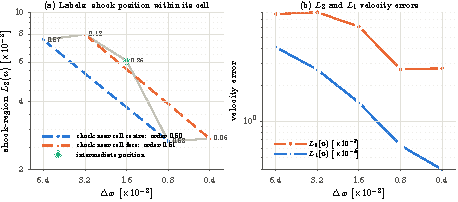
\includegraphics[width=\textwidth]{G11_shock_phase.pdf}
\caption{(a) Velocity error in the cells surrounding the shock, labelled with the position
of the exact shock within its cell.  (b) Global $L_2$ and $L_1$ velocity errors.}
\label{fig:phase}
\end{figure}

\begin{figexplain}{\Cref{fig:phase}}
\begin{fx}
\item[What is shown.] Panel (a) shows the $L_2$ velocity error contributed by the eight cells
  around the shock.  Each point is labelled with the fractional position of the exact shock
  inside its cell (0 = at a cell face, 0.5 = at the cell centre).  Panel (b) compares the
  global $L_2$ and $L_1$ velocity errors.
\item[How to read it.] Grids on which the shock falls at a similar position within a cell are
  joined by the same coloured line; the legend reports the observed order along each line.
\item[What it means.] Between 93\% and 99\% of the velocity $L_2$ error comes from the cells
  at the shock, where the velocity drops from 0.93 to 0.  The size of that error depends on
  whether the exact shock lies near a cell face or near a cell centre, and this position
  differs from grid to grid.  When grids with comparable shock positions are compared, the
  error decreases at the expected order of about 0.5.  The apparent stall of $L_2(u)$
  between 25{,}000 and 50{,}000 cells is therefore an artefact of the error measurement, not
  a limitation of the solver.  The $L_1$ velocity error, which is less sensitive to a few
  cells, decreases steadily with order 0.89.
\end{fx}
\end{figexplain}

\subsection{Contact and shock thickness; influence of the relaxation time}
\label{sec:tau}

\begin{figure}[H]
\centering
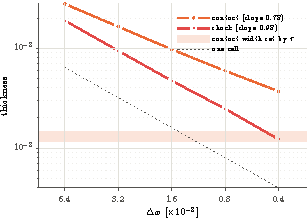
\includegraphics[width=0.7\textwidth]{G14_feature_thickness.pdf}
\caption{Measured thickness of the contact and the shock versus cell size.  The shaded band
is the contact width set by the relaxation time $\tau$.}
\label{fig:thick}
\end{figure}

\begin{figexplain}{\Cref{fig:thick}}
\begin{fx}
\item[What is shown.] The thickness of each discontinuity, defined as its jump divided by the
  steepest computed gradient, for each grid.  The dotted line marks a thickness of one cell;
  the shaded band marks the physical contact width produced by $\tau = 5\times10^{-6}$.
\item[How to read it.] A slope of 1 means the feature always occupies the same number of
  cells.  A feature that reached the shaded band would be limited by the physics of the
  model rather than by the grid.
\item[What it means.] The shock has slope 0.98 and spans about three cells on every grid, as
  expected for a captured shock.  The contact has slope 0.73, close to the theoretical 2/3
  for a second-order scheme, and grows from 4 to 9 cells across the grid sequence.  On the
  finest grid the contact is still about three times wider than its physical ($\tau$-set)
  width, so the present results are limited by grid resolution rather than by $\tau$.
  Extrapolating the measured trend, the two widths would become equal at about
  $2\times10^{5}$ cells.
\end{fx}
\end{figexplain}

The influence of $\tau$ is confirmed by comparison with an earlier study at a ten times
larger relaxation time ($\tau = 5\times10^{-5}$; \cref{tab:tau}).  With the larger $\tau$ the
contact is naturally about three times wider, and the density error stopped decreasing
at approximately $1.13\times10^{-3}$ beyond 40{,}000 cells.  With the present value it
continues to decrease.  The earlier runs also used a larger time step, so this comparison
changes two parameters at once.

\begin{table}[H]
\centering
\caption{Global $L_2$ density error for two relaxation times.}
\label{tab:tau}
\small
\begin{tabular}{@{}rccc@{}}
\toprule
$N_x$ & $\tau = 5\times10^{-5}$ (earlier study) & $\tau = 5\times10^{-6}$ (present) & Ratio \\
\midrule
3,125  & $3.24\times10^{-3}$ & $3.16\times10^{-3}$ & 0.97 \\
6,250  & $1.96\times10^{-3}$ & $1.81\times10^{-3}$ & 0.92 \\
12,500 & $1.59\times10^{-3}$ & $1.39\times10^{-3}$ & 0.87 \\
25,000 & $1.26\times10^{-3}$ & $1.00\times10^{-3}$ & 0.80 \\
40,000 & $1.13\times10^{-3}$ & --- & --- \\
50,000 & $1.13\times10^{-3}$ & $0.78\times10^{-3}$ & 0.69 \\
\bottomrule
\end{tabular}
\end{table}

\subsection{Limiter comparison}
\label{sec:limiters}

Five limiters developed during the project were compared on 6{,}250 cells with all other
settings identical (\cref{tab:lim,fig:limprof}).  The two ``hybrid'' limiters switched
between MC and minmod, either separately for each population or using a shared indicator
based on density, pressure and temperature.

\begin{table}[H]
\centering
\caption{Limiter comparison on 6{,}250 cells.  Lower values are better in every column.}
\label{tab:lim}
\small
\begin{tabular}{@{}lccccc@{}}
\toprule
Limiter & $L_1(\rho)$ & $L_1(u)$ & $L_1(p)$ & $L_1(T)$ & $T$ overshoot \\
\midrule
Minmod                          & 1.68e-4 & 3.36e-4 & 1.42e-4 & 2.65e-4 & 4.5e-4 \\
MC                              & 1.06e-4 & 2.07e-4 & 8.86e-5 & 1.68e-4 & 6.7e-3 \\
Population hybrid               & 1.34e-4 & 2.89e-4 & 1.14e-4 & 2.16e-4 & 2.6e-3 \\
Macroscopic hybrid              & 1.64e-4 & 3.27e-4 & 1.35e-4 & 2.66e-4 & 6.2e-4 \\
\rowcolor{blue!6}Generalized minmod, $\theta=1.2$ & 1.30e-4 & 2.69e-4 & 1.09e-4 & 2.08e-4 & 1.6e-3 \\
\bottomrule
\end{tabular}
\end{table}

\begin{figure}[H]
\centering
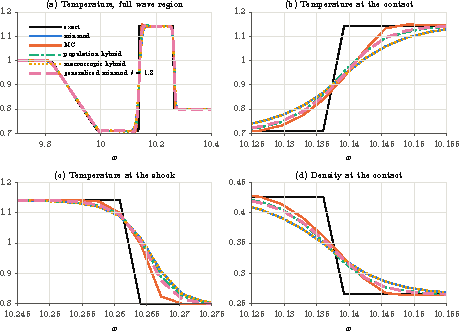
\includegraphics[width=\textwidth]{G12_limiter_profiles.pdf}
\caption{Temperature and density profiles near the contact and shock for the five
limiters on 6{,}250 cells.}
\label{fig:limprof}
\end{figure}

\begin{figexplain}{\Cref{fig:limprof}}
\begin{fx}
\item[What is shown.] Panel (a) shows temperature over the whole wave region; panels (b)--(d)
  magnify the temperature at the contact and the shock, and the density at the contact.
\item[How to read it.] A curve that rises more steeply is sharper (less diffusive).  A curve
  that rises above the black exact value just behind the contact is overshooting.
\item[What it means.] MC (orange) is the sharpest but exceeds the exact post-contact
  temperature, an overshoot of $6.7\times10^{-3}$.  Minmod (blue) and the macroscopic hybrid
  (nearly identical to minmod) do not overshoot but are the most diffused.  Generalized minmod
  with $\theta = 1.2$ (pink dashed) is visibly sharper than minmod while keeping the
  overshoot small: it lowers all four $L_1$ errors by 20--23\% relative to minmod and
  reduces the MC overshoot by 77\%.
\end{fx}
\end{figexplain}

\subsection{Selection of the limiter parameter $\theta$}

\begin{figure}[H]
\centering
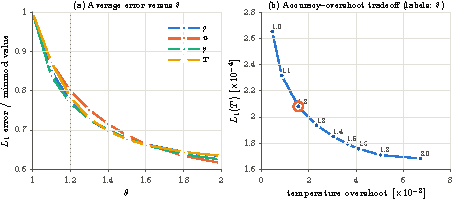
\includegraphics[width=\textwidth]{G13_theta_tradeoff.pdf}
\caption{Effect of $\theta$ on average error (a) and the tradeoff between temperature error
and temperature overshoot (b), on 6{,}250 cells.}
\label{fig:theta}
\end{figure}

\begin{figexplain}{\Cref{fig:theta}}
\begin{fx}
\item[What is shown.] Nine values of $\theta$ between 1 (minmod) and 2 (MC).  Panel (a) shows
  each variable's $L_1$ error relative to its minmod value; panel (b) plots the temperature
  error against the temperature overshoot, with each point labelled by $\theta$.
\item[How to read it.] In (a), lower is better.  In (b), the ideal point would be the lower-left
  corner (small error and small overshoot); the circled point is $\theta = 1.2$.
\item[What it means.] Increasing $\theta$ always reduces the average error and always
  increases the overshoot; no value is best in both respects.  The curve in (b) is steep at
  small $\theta$, so the first increments of $\theta$ buy large accuracy gains at little
  overshoot cost.  $\theta = 1.2$ obtains 59\% of the error reduction available between
  minmod and MC while incurring 18\% of the overshoot increase.  On finer grids the overshoot
  at $\theta = 1.2$ disappears entirely (\cref{fig:zoom}d), making it a sound working choice.
\end{fx}
\end{figexplain}

% ===========================================================================
\section{Conclusions and recommendations}
\label{sec:conclusions}
% ===========================================================================

\begin{enumerate}
  \item The D1V5 finite-volume DBM solves the Sod problem accurately and robustly: no
        oscillations, no stability interventions, and conservation of mass and energy to
        $10^{-12}$ on all grids.
  \item The observed orders ($L_1$: 0.81--0.89; $L_2$: 0.40--0.63) are below first order in
        the strict sense, but they match a conventional second-order Euler solver on the same
        grids and clearly exceed first-order methods ($L_1$ order 0.64); this is the expected
        behaviour of a second-order scheme on a solution with a shock and a contact.
  \item The contact discontinuity limits convergence; the shock remains about three cells
        wide on every grid.  At $\tau = 5\times10^{-6}$ the results remain grid-limited up to
        50{,}000 cells.
  \item At equal resolution the DBM and a conventional second-order Euler solver achieve
        similar accuracy, but the DBM is 100 to 800 times more expensive because its
        explicit collision term restricts the time step to $\tau/4$; the cost per time step
        is comparable.  The method's advantage lies in
        its kinetic (non-equilibrium) information rather than in efficiency for purely
        inviscid problems.
  \item Generalized minmod with $\theta = 1.2$ provides a balanced compromise between
        numerical diffusion and temperature overshoot.
\end{enumerate}

\paragraph{Recommendations.}
\begin{itemize}
  \item Remove the collision limit on the time step, either by treating the collision term
        implicitly with an IMEX Runge--Kutta scheme~\citep{PareschiRusso2005} or by adopting
        a scheme that couples transport and collision, such as the discrete unified
        gas-kinetic scheme~\citep{Guo2013}.  The time step would then be set by the transport
        CFL condition rather than by $\tau$.
  \item Perform a single time-step-halving test on the finest grid to confirm that temporal
        error is negligible.
  \item Verify formal second-order accuracy on a smooth test problem, such as a
        small-amplitude acoustic pulse, which the Sod problem cannot demonstrate.
  \item Report velocity convergence using the $L_1$ norm, or with grid sequences that sample
        different shock positions, to avoid the measurement effect of \cref{sec:phase}.
  \item Before extending the method to two dimensions, select a velocity set whose slowest
        speed exceeds the expected flow velocities.
\end{itemize}

% ===========================================================================
\section*{Nomenclature}
% ===========================================================================
\begin{small}
\begin{tabularx}{\textwidth}{@{}l X l X@{}}
$c_i$ & discrete particle velocity & $p$ & pressure \\
$f_i$ & population (distribution) $i$ & $T$ & temperature \\
$\feq_i$ & equilibrium population & $u$ & flow velocity \\
$\tau$ & relaxation time & $\rho$ & density \\
$\eta_0$ & internal-energy parameter & $\gamma$ & ratio of specific heats \\
$\Delta x$, $N_x$ & cell size, number of cells & $\Delta t$ & time step \\
$\theta$ & limiter parameter & CFL & Courant number \\
$L_1$, $L_2$ & mean-absolute and RMS errors & $p$ & also: observed order of accuracy \\
\end{tabularx}
\end{small}

% ===========================================================================
\begin{thebibliography}{99}
\small
\bibitem{BGK1954}
P.~L. Bhatnagar, E.~P. Gross, and M.~Krook, ``A model for collision processes in gases. I,''
\emph{Physical Review} \textbf{94}, 511--525 (1954).
\href{https://doi.org/10.1103/PhysRev.94.511}{doi:10.1103/PhysRev.94.511}

\bibitem{ChapmanCowling1970}
S.~Chapman and T.~G. Cowling, \emph{The Mathematical Theory of Non-uniform Gases}, 3rd ed.,
Cambridge University Press (1970).

\bibitem{Gottlieb2001}
S.~Gottlieb, C.-W. Shu, and E.~Tadmor, ``Strong stability-preserving high-order time
discretization methods,'' \emph{SIAM Review} \textbf{43}, 89--112 (2001).
\href{https://doi.org/10.1137/S003614450036757X}{doi:10.1137/S003614450036757X}

\bibitem{Greenough2004}
J.~A. Greenough and W.~J. Rider, ``A quantitative comparison of numerical methods for the
compressible Euler equations: fifth-order WENO and piecewise-linear Godunov,''
\emph{Journal of Computational Physics} \textbf{196}, 259--281 (2004).
\href{https://doi.org/10.1016/j.jcp.2003.11.002}{doi:10.1016/j.jcp.2003.11.002}

\bibitem{Guo2013}
Z.~Guo, K.~Xu, and R.~Wang, ``Discrete unified gas kinetic scheme for all Knudsen number
flows: low-speed isothermal case,'' \emph{Physical Review E} \textbf{88}, 033305 (2013).
\href{https://doi.org/10.1103/PhysRevE.88.033305}{doi:10.1103/PhysRevE.88.033305}

\bibitem{Harten1977}
A.~Harten, ``The artificial compression method for computation of shocks and contact
discontinuities. I. Single conservation laws,'' \emph{Communications on Pure and Applied
Mathematics} \textbf{30}, 611--638 (1977).
\href{https://doi.org/10.1002/cpa.3160300506}{doi:10.1002/cpa.3160300506}

\bibitem{Harten1983}
A.~Harten, ``High resolution schemes for hyperbolic conservation laws,'' \emph{Journal of
Computational Physics} \textbf{49}, 357--393 (1983).
\href{https://doi.org/10.1016/0021-9991(83)90136-5}{doi:10.1016/0021-9991(83)90136-5}

\bibitem{JiangShu1996}
G.-S. Jiang and C.-W. Shu, ``Efficient implementation of weighted ENO schemes,''
\emph{Journal of Computational Physics} \textbf{126}, 202--228 (1996).
\href{https://doi.org/10.1006/jcph.1996.0130}{doi:10.1006/jcph.1996.0130}

\bibitem{KataokaTsutahara2004Euler}
T.~Kataoka and M.~Tsutahara, ``Lattice Boltzmann method for the compressible Euler
equations,'' \emph{Physical Review E} \textbf{69}, 056702 (2004).
\href{https://doi.org/10.1103/PhysRevE.69.056702}{doi:10.1103/PhysRevE.69.056702}

\bibitem{KurganovTadmor2000}
A.~Kurganov and E.~Tadmor, ``New high-resolution central schemes for nonlinear conservation
laws and convection--diffusion equations,'' \emph{Journal of Computational Physics}
\textbf{160}, 241--282 (2000).
\href{https://doi.org/10.1006/jcph.2000.6459}{doi:10.1006/jcph.2000.6459}

\bibitem{LeVeque2002}
R.~J. LeVeque, \emph{Finite Volume Methods for Hyperbolic Problems}, Cambridge University
Press (2002).
\href{https://doi.org/10.1017/CBO9780511791253}{doi:10.1017/CBO9780511791253}

\bibitem{LiskaWendroff2003}
R.~Liska and B.~Wendroff, ``Comparison of several difference schemes on 1D and 2D test
problems for the Euler equations,'' \emph{SIAM Journal on Scientific Computing}
\textbf{25}, 995--1017 (2003).
\href{https://doi.org/10.1137/S1064827502402120}{doi:10.1137/S1064827502402120}

\bibitem{PareschiRusso2005}
L.~Pareschi and G.~Russo, ``Implicit--explicit Runge--Kutta schemes and applications to
hyperbolic systems with relaxation,'' \emph{Journal of Scientific Computing} \textbf{25},
129--155 (2005).
\href{https://doi.org/10.1007/s10915-004-4636-4}{doi:10.1007/s10915-004-4636-4}

\bibitem{ShuOsher1988}
C.-W. Shu and S.~Osher, ``Efficient implementation of essentially non-oscillatory
shock-capturing schemes,'' \emph{Journal of Computational Physics} \textbf{77}, 439--471
(1988).
\href{https://doi.org/10.1016/0021-9991(88)90177-5}{doi:10.1016/0021-9991(88)90177-5}

\bibitem{Sod1978}
G.~A. Sod, ``A survey of several finite difference methods for systems of nonlinear
hyperbolic conservation laws,'' \emph{Journal of Computational Physics} \textbf{27}, 1--31
(1978).
\href{https://doi.org/10.1016/0021-9991(78)90023-2}{doi:10.1016/0021-9991(78)90023-2}

\bibitem{Sweby1984}
P.~K. Sweby, ``High resolution schemes using flux limiters for hyperbolic conservation
laws,'' \emph{SIAM Journal on Numerical Analysis} \textbf{21}, 995--1011 (1984).
\href{https://doi.org/10.1137/0721062}{doi:10.1137/0721062}

\bibitem{Toro2009}
E.~F. Toro, \emph{Riemann Solvers and Numerical Methods for Fluid Dynamics}, 3rd ed.,
Springer (2009).
\href{https://doi.org/10.1007/b79761}{doi:10.1007/b79761}

\bibitem{ToroSpruceSpeares1994}
E.~F. Toro, M.~Spruce, and W.~Speares, ``Restoration of the contact surface in the
HLL-Riemann solver,'' \emph{Shock Waves} \textbf{4}, 25--34 (1994).
\href{https://doi.org/10.1007/BF01414629}{doi:10.1007/BF01414629}

\bibitem{vanLeer1977}
B.~van Leer, ``Towards the ultimate conservative difference scheme. IV. A new approach to
numerical convection,'' \emph{Journal of Computational Physics} \textbf{23}, 276--299 (1977).
\href{https://doi.org/10.1016/0021-9991(77)90095-X}{doi:10.1016/0021-9991(77)90095-X}

\bibitem{vanLeer1979}
B.~van Leer, ``Towards the ultimate conservative difference scheme. V. A second-order
sequel to Godunov's method,'' \emph{Journal of Computational Physics} \textbf{32}, 101--136
(1979).
\href{https://doi.org/10.1016/0021-9991(79)90145-1}{doi:10.1016/0021-9991(79)90145-1}

\bibitem{XuZhangZhang2018}
A.~Xu, G.~Zhang, and Y.~Zhang, ``Discrete Boltzmann modeling of compressible flows,'' in
\emph{Kinetic Theory}, G.~Z. Kyzas and A.~C. Mitropoulos (eds.), InTech (2018);
\href{https://arxiv.org/abs/1708.09187}{arXiv:1708.09187}.
\end{thebibliography}

\end{document}
